\documentclass{standalone}
\usepackage{pgfplots}
\usepgfplotslibrary{fillbetween}

\pgfplotsset{width=10cm,compat=1.15}

\pagestyle{empty}
\begin{document}
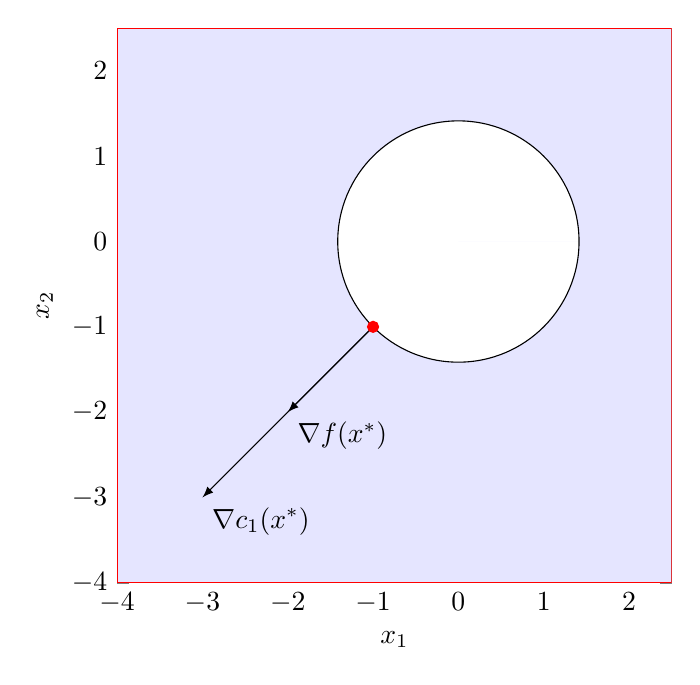
\begin{tikzpicture}
    \begin{axis}[%
        xmin=-4,%
        xmax=2.5,%
        ymin=-4,%
        ymax=2.5,%
        axis equal image,%
        xlabel={$x_1$},%
        ylabel={$x_2$},%
        axis background/.style={even odd rule, insert path={(0,0) circle[radius=2^0.5]}},%
 ]  
    
        \path[draw,red,name path=L1](current axis.south west) rectangle (current axis.north east);
        \draw[name path=L2](axis cs:0,0) circle[radius=2^0.5];
        \draw[-latex] (axis cs:-1,-1) -- (axis cs:-3,-3) node[below right] {$\nabla c_1(x^{\ast})$};
        \draw[-latex] (axis cs:-1,-1) -- (axis cs:-2,-2) node[below right] {$\nabla f(x^{\ast})$};
        \addplot[red,mark=*,only marks] coordinates {(-1,-1)};
        \addplot[blue!10] fill between[of=L1 and L2];
    \end{axis}
\end{tikzpicture}
\end{document} 